\section{Disabled C-States}

Next, up, experiment \#2 will be covered, where the DUT was in performance mode. This was done to attempt to get a more realistic idle case, resulting in a more realistic dynamic energy consumption of the other test cases.

\subsection{Expectations} 

The expectation for this experiment, is a higher energy consumption on all test cases, especially the idle test case. This increased energy consumption for the test cases will most likely result in a decreased dynamic energy consumption, as we expect the energy consumption for the idle test case to increase more than the other test cases. In addition to this, the expection will also be a lower standard deviation for especially the clamp.

\subsection{Result} 
When considering the result, the test case Nbody can be seen in \cref{fig:Nbody_Cores_comparison_dynamic_energy_without_outliers_avg_watts_exp2}, and for the other test cases in \cref{app:exp_two}. In this graph, the measurements from the first and second experiments can be observed and compared. The results will be discussed through \textbf{RQ2} and \textbf{3}.

\paragraph*{RQ1:} When comparing based on the different measuring instruments, the patterns and orders of the profilers has not changed, but the dynamic energy consumption has. This is especially for the clamp on windows, where the uncertainty has decreased in all cases except for BinaryTrees, where it increased. IPG and LHM are still similar, and still measures a higher values compared to the clam on windows. When comparing IPG and LHM to RAPL, RAPL now reports a higher energy consumption in all cases, as a very limited effect on the reported measurements when disabling the C-states is observed for RAPL.

\paragraph*{RQ2:} When comparing Windows and Linux, the difference between an enabled and disabled C-state can be observed for Nbody in \cref{fig:Nbody_Cores_comparison_dynamic_energy_without_outliers_avg_watts_exp2} and all other test cases in \cref{app:exp_two}. The effect for Linux in general is limited, especially on RAPL. When considering the clamp on Linux it has improved in some cases. For Nbody, the min/max values are now very close the the 25th and 75th percentile, but the dynamic energy consumption is still close to the same value, but for Fasta, a very limited effect is observed. On windows it is different, where the dynamic energy for all measurement instruments has decreased. This is especially clear for the clamp in Windows, where the uncertainty before was the highest of all measuring instruments.


                \begin{figure}[H]
                    \centering
                    \begin{tikzpicture}
                        \pgfplotsset{%
                            width=1\textwidth,
                            height=0.4\textheight
                        }
                        \begin{axis}[
                            xlabel={Start battery level},
                            ylabel={Average dynamic energy (watt)},
                            ymin=0,ymax=20,
                        ]
                        
                            \addplot [mark=none, ultra thick, red]  coordinates {
                            (40, 0.006595684402444291)(45, 0.007295220674193181)(50, 0.007999659608910881)(55, 0.007202467971243639)(60, 0.007280865079495958)(65, 0.006858423509955077)(70, 0.008369444141141925)(75, 0.007144940647010992)(80, 0.004753236834232667)
                            };
                            \addlegendentry{Surface4Pro - IntelPowerGadget}
                            
                            \addplot [mark=none, ultra thick, blue]  coordinates {
                            (40, 0.002385328427460912)(45, 0.0017856511573015649)(50, 0.0025901992189954056)(55, 0.00210998144366709)(60, 0.00286452646862575)(65, 0.0020038487280194628)(70, 0.002908483770774353)(75, 0.0005098111150931342)(80, -0.005995916826693459)
                            };
                            \addlegendentry{Surface4Pro - HardwareMonitor}
                            
                            \addplot [mark=none, ultra thick, orange]  coordinates {
                            (50, 251.8661014299577)(55, 214.7597259251014)(60, 162.23880995564176)(65, 107.43421593849766)(70, 53.9187387386668)(75, 0.7554852536149699)(80, -44.463085003568885)
                            };
                            \addlegendentry{Surface4Pro - RAPL}
                            
                            \addplot [mark=none, dashdotted, red]  coordinates {
                            (40, -0.004038062354887025)(45, -0.004312668500277529)(50, -0.003808663911021498)(55, -0.0037057407527755254)(60, -0.004478257932982471)(65, -0.0026308734995501644)(70, -0.0034090674446925874)(75, -0.003041497079697436)(80, -0.0020334307266356875)
                            };
                            \addlegendentry{SurfaceBook - IntelPowerGadget}
                            
                            \addplot [mark=none, dashdotted, blue]  coordinates {
                            (40, -0.002443518930616523)(45, -0.0029256880137447055)(50, -0.002551777773312929)(55, -0.0027567211782433486)(60, -0.002206859154402231)(65, -0.0026388300848279207)(70, -0.0024597736945479324)(75, -0.002445350799195827)(80, -0.000541271265011134)
                            };
                            \addlegendentry{SurfaceBook - HardwareMonitor}
                            
                            \addplot [mark=none, dashdotted, orange]  coordinates {
                            (40, 101.92702155010147)(45, 86.7212700795567)(50, 69.40754598562454)(55, 51.343785407669614)(60, 32.443112755251185)(65, 14.52577919077786)(70, -4.520517378551423)(75, -23.811706977384954)(80, -35.700372165212755)
                            };
                            \addlegendentry{SurfaceBook - RAPL}
                            
                        \end{axis}
                    \end{tikzpicture} 
                \caption{A graph illustrating the energy consumption of Dram for test case Nbody with regards to the battey level of the DUT (with outliers)} \label{fig:Nbody_Dram_charge}
                \end{figure}
                
% 
            \begin{figure}
                \centering
                \begin{tikzpicture}
                    \pgfplotsset{%
                        width=1\textwidth,
                        height=0.5\textheight
                    }
                    \begin{axis}[
                        xlabel={Start temperature},
                        ylabel={Average dynamic energy (watt)},
                    ]
                    
                    \end{axis}
                \end{tikzpicture} 
            \caption{A graph illustrating the energy consumption of Cores for test case TestCaseIdle with regards to the temperature of the DUT} \label{fig:TestCaseIdle_Cores}
            \end{figure}
            
% 
                            \begin{figure}
                                \centering
                                \begin{tikzpicture}[]
                                    \pgfplotsset{%
                                        width=.85\textwidth,
                                        height=.15\textheight
                                    }
                                    \begin{axis}[xlabel={Average energy consumption (Watts)}, title={Cores - BinaryTrees - Energy - without outliers}, ytick={},
                                    yticklabels={
                                        
                                        },
                                        xmin=0,xmax=20,
                                        ]
                                    
                                    \end{axis}
                                \end{tikzpicture}
                            \caption{A comparison of of Cores energy consumption for test case BinaryTrees for the Surface4Pro,  experiment \#2 (without outliers)} \label{fig:BinaryTrees_Cores_comparison_energy_without_outliers_Surface4Pro_avg_watts_exp2}
                            \end{figure}
                            

